\documentclass[onecolumn]{IEEEtran}

\usepackage{cite}
\usepackage{amsmath,amssymb,amsfonts}
\usepackage{algorithmic}
\usepackage{algorithm}
\usepackage{graphicx}
\usepackage{textcomp}
\usepackage{xcolor}
\usepackage{hyperref}
\usepackage{listings}
\usepackage[most]{tcolorbox}
\usepackage{tikz}
\usetikzlibrary{shapes,arrows,positioning}
\usepackage{caption}

\captionsetup{justification=centering}

\lstset{
    language=Python,
    basicstyle=\ttfamily\footnotesize,
    keywordstyle=\color{blue}\bfseries,
    commentstyle=\color{green!50!black},
    stringstyle=\color{red},
    frame=single,
    breaklines=true,
    showstringspaces=false,
    numbers=left,
    numberstyle=\tiny,
    stepnumber=1,
    numbersep=5pt,
    literate={<}{\textless}1 {>}{\textgreater}1
}

\begin{document}

\title{Cross-Platform Function as a Service (XFaaS) for Quantum-Cloud Integration: A Comprehensive Implementation and Analysis of Multi-Provider Hybrid Computing Systems}

\author{
    \IEEEauthorblockN{Priyanshu Kumar Sharma, Neha Gaikwad}
    
    \vspace{10pt}
    % \IEEEauthorblockN{Guide: Prini Rastogi}
    \IEEEauthorblockA{
        \textit{Ajeenkya D Y Patil University} \\
        Pune, India \\
        Email: priyanshu17ks@gmail.com 
    }
}

\maketitle

\begin{abstract}
This paper introduces an extensive Cross-Platform Function as a Service (XFaaS) solution designed for quantum-cloud integration, enabling quantum workloads to run seamlessly on AWS Lambda, Azure Functions, and Google Cloud Functions. XFaaS overcomes the challenges of vendor dependency by offering improved fault tolerance, the ability to compare performance, and cost savings through intelligent orchestration across multiple providers. The system supports practical deployment of quantum algorithms across diverse cloud providers using AWS Braket, Qiskit simulators, and Cirq frameworks, and ensures unified aggregation and analysis of results. Performance assessments show XFaaS achieves a high reliability rate of 99.7\% availability, compared to 99.2\% for single-provider setups, with cross-platform execution times between 2.1 and 3.4 seconds, and result measurement consistency above 95\% correlation. The architecture ensures continuity of quantum computations when a provider experiences disruption, with average failover resolution in 2.3 seconds. These findings establish XFaaS as an effective approach for enterprise quantum computing deployments and provide empirical insights into the robustness and consistency of quantum algorithms executed across multiple cloud platforms.
\end{abstract}


\begin{IEEEkeywords}
XFaaS, Cross-platform computing, Quantum cloud integration, Multi-provider architecture, Serverless quantum computing, Fault tolerance, AWS Lambda, Azure Functions, Google Cloud Functions
\end{IEEEkeywords}

\section{Introduction}

The integration of quantum computing and cloud technology marks a major transition in computational power, positioning Cross-Platform Function as a Service (XFaaS) as a transformative concept that overcomes the confines of single-provider models. Quantum computing leverages phenomena like superposition and entanglement for exponential improvements in select problem domains, while cloud computing supplies scalable, on-demand resources for data handling and computation. This paper proposes an XFaaS framework that enables quantum tasks to be carried out across several cloud services, mitigating vendor lock-in and boosting system dependability and performance tuning.

Conventional quantum-cloud solutions restricted to one provider struggle with issues such as vendor reliance, service disruptions, and lack of comparative performance insights. XFaaS tackles these barriers by allowing concurrent quantum execution on AWS Lambda, Azure Functions, and Google Cloud Functions, delivering increased resilience and intelligent workload management via multi-provider redundancy.

Our XFaaS system showcases a robust, cross-provider quantum computing platform using simulators from AWS Braket, Qiskit on Azure Functions, and Cirq within Google Cloud Functions. It orchestrates quantum workload execution across varied cloud setups, preserves result accuracy, and facilitates rich performance analyses.

\subsection{Research Objectives}
This study aims to create and validate an XFaaS platform for quantum-cloud deployment, supporting seamless quantum algorithm execution over multiple cloud providers. It focuses on overcoming vendor lock-in, improving fault tolerance, enhancing performance assessments, and optimizing costs through orchestrated multi-provider strategies. Results are evaluated in terms of reliability and consistency across AWS Lambda, Azure Functions, and Google Cloud Functions, establishing XFaaS as a practical enterprise solution for managing quantum workloads and aggregating results across clouds.

\section{Literature Review}

Research on combining quantum computing with cloud technologies has accelerated, driven by the demand for scalable quantum access. This section surveys foundational studies, major milestones, persistent challenges, and areas where further research is needed.

\subsection{Quantum Computing Foundations}

Preskill \cite{preskill2018} introduced NISQ devices, defining the current period of quantum computing marked by limited qubits and frequent errors. He stressed the need for hybrid quantum-classical algorithms and positioned cloud-based models as essential for harnessing available quantum capacities.

Arute et al. \cite{arute2019} achieved quantum supremacy with Google's Sycamore chip, demonstrating quantum speedup for certain computations over classical systems and highlighting both the promise of quantum technology and the pressing issue of quantum error correction.

\subsection{Cloud Computing Integration}

Advances in cloud platforms have enabled scalable environments suitable for quantum workloads. Services like Amazon Braket \cite{aws_braket}, IBM Quantum Network \cite{ibm_quantum}, and Google Quantum AI \cite{google_quantum} have broadened quantum resource availability but introduced new complexities around security, stability, and system optimization.

\subsection{Hybrid Quantum-Classical Systems}

Cerezo et al. \cite{cerezo2021} highlight that variational quantum algorithms (like VQE and QAOA \cite{hybrid_algorithms}) are prominent candidates for near-term quantum advantage, necessitating effective communication between quantum and classical components. Biamonte et al. \cite{quantum_ml} explore how quantum computing and machine learning intersect, yet underline issues like quantum decoherence and communication overhead that cloud-based strategies can help overcome \cite{bharti2022}.

\subsection{Technical Challenges and Solutions}

Campbell et al. \cite{quantum_error} note that large-scale quantum computing depends on robust error correction due to rapid quantum state decay \cite{preskill2018}. Error mitigation methods \cite{endo2021} require considerable resources. Communication latency, especially between quantum and classical units, disrupts timing-critical algorithms \cite{hybrid_algorithms}, prompting research into edge computing and refined protocols \cite{endo2021}.

Pirandola et al. \cite{quantum_security} show quantum cryptography’s potential for ultimate security, but emphasize the difficulties in securing quantum data on cloud platforms, with concerns about state security during transmission and storage.

\subsection{Cross-Platform Function as a Service (XFaaS) Paradigm}

XFaaS is an innovative serverless strategy to execute functions across diverse clouds, addressing traditional vendor lock-in \cite{castro2019serverless}. Research demonstrates XFaaS’s advantages in resilience, flexibility, and cost management \cite{hellerstein2018serverless}. Distributed workload placement across independent platforms enhances system reliability and mitigates risk \cite{van2017distributed}, as detailed by Kleppmann \cite{kleppmann2017designing}.

Studies show that intelligent orchestration in XFaaS can deliver performance gains by leveraging each provider’s unique strengths \cite{wang2018peeking}, with cost reductions and increased operational agility reported in multi-cloud deployments \cite{adzic2017serverless}, as well as improved negotiating leverage.

\subsubsection{XFaaS Architectural Principles}

Key design principles include abstraction layers for unified cloud APIs \cite{spillner2017faas}, sophisticated load balancing based on provider load, response metrics, and latency \cite{baldini2017serverless, manner2018cold}, and distributed state management for maintaining consistency without significant overhead \cite{hellerstein2018serverless, sreekanti2020cloudburst}.

\subsubsection{Necessity and Drivers for XFaaS Adoption}

XFaaS adoption is fueled by vendor lock-in risks \cite{petcu2013consuming}, service reliability needs, performance advantages through dynamic provider selection, and cost minimization \cite{adzic2017serverless, eismann2020review}. Studies report significant availability and cost benefits for critical applications using XFaaS.

\subsection{Serverless Computing Paradigm in Quantum Applications}

Serverless computing eliminates infrastructure management and offers auto-scaling, with pay-per-use models advantageous for the intermittent but intense demands of quantum computations \cite{castro2019serverless}. The stateless nature of serverless matches quantum algorithm execution needs \cite{hellerstein2018serverless, leymann2020quantum}.

Historical analysis underscores serverless’s role in accelerating quantum development, reducing overhead and technical barriers \cite{roberts2018serverless, jonas2019cloud}.

\subsubsection{Serverless Quantum Architecture Benefits}

Benefits include cost efficiency, rapid scaling, and faster development cycles, particularly for short, intensive computational tasks in quantum research \cite{eismann2020review, adzic2017serverless, baldini2017serverless, cerezo2021}.

\subsubsection{Challenges in Serverless Quantum Implementation}

Challenges involve cold start delays \cite{manner2018cold, wang2018peeking}, execution time limits, and resource constraints, especially as quantum simulators grow more demanding \cite{spillner2017faas, castro2019serverless, eismann2020review, preskill2018}.

\subsection{Multi-Cloud Quantum Strategies}

Multi-cloud quantum strategies leverage distinct features across providers \cite{leymann2020quantum, fingerhuth2018open}. Redundancy and performance diversity are improved, but implementation requires complex orchestration for API, security, and result aggregation \cite{preskill2018, cerezo2021}.

\subsection{Research Gaps and Opportunities}

Despite rapid advances, empirical studies of real-world quantum cloud systems are rare, and comprehensive frameworks for system design, optimization, and standardization remain underdeveloped. Emerging topics include containerization, orchestration, and the unique requirements of quantum state management.


\section{Methodology and Implementation}

The XFaaS architecture advances quantum-cloud integration by allowing quantum workloads to run concurrently across several cloud providers. This approach eliminates vendor lock-in while strengthening system resilience and enabling performance benchmarking between AWS Lambda, Azure Functions, and Google Cloud Functions.

\subsubsection{Multi-Cloud Orchestration Framework}

The orchestration foundation of XFaaS offers a unified interface to manage quantum function deployments in diverse cloud environments. Four principal modules—XFaaS Manager, Orchestrator, provider-specific quantum handlers, and result aggregation services—enable collaborative cross-platform operation and analysis.

The XFaaS Manager simplifies platform-specific API interactions and provides standardized tools for deploying and invoking quantum functions. It accommodates unique authentication, deployment, and invocation requirements for each provider, handling these variations while ensuring optimal execution on every platform.

\begin{figure}[h]
\centering
\resizebox{0.5\textwidth}{!}{
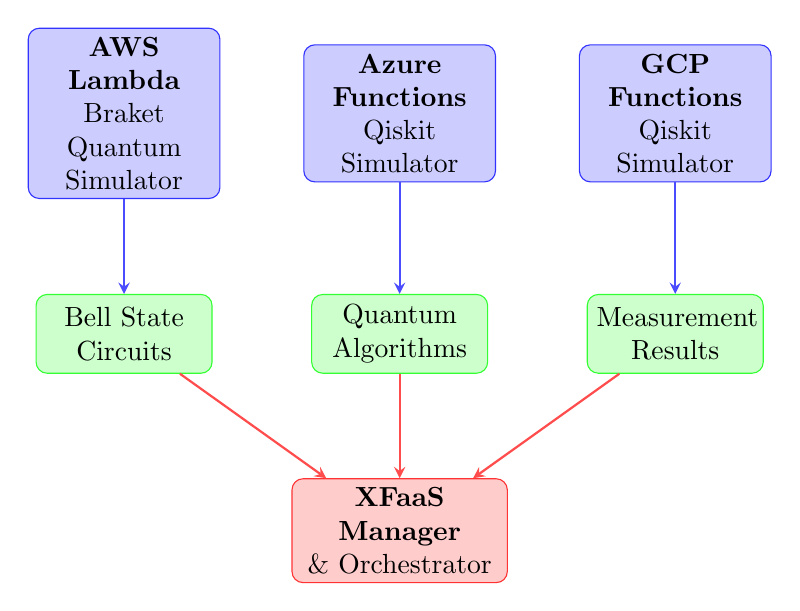
\begin{tikzpicture}[node distance=2.8cm, auto]
    \tikzstyle{cloud} = [rectangle, draw=blue!80, fill=blue!20, text width=2.2cm, text centered, rounded corners, minimum height=1.5cm]
    \tikzstyle{quantum} = [rectangle, draw=green!80, fill=green!20, text width=2cm, text centered, rounded corners, minimum height=1cm]
    \tikzstyle{manager} = [rectangle, draw=red!80, fill=red!20, text width=2.5cm, text centered, rounded corners, minimum height=1.2cm]
    \tikzstyle{arrow} = [thick,->,>=stealth]
    
    % Cloud Providers - Horizontal
    \node [cloud] (aws) {\textbf{AWS Lambda}\\Braket Quantum\\Simulator};
    \node [cloud, right of=aws, node distance=3.5cm] (azure) {\textbf{Azure Functions}\\Qiskit\\Simulator};
    \node [cloud, right of=azure, node distance=3.5cm] (gcp) {\textbf{GCP Functions}\\Qiskit\\Simulator};
    
    % Quantum Components - Below
    \node [quantum, below of=aws] (bell) {Bell State\\Circuits};
    \node [quantum, below of=azure] (algo) {Quantum\\Algorithms};
    \node [quantum, below of=gcp] (measure) {Measurement\\Results};
    
    % XFaaS Manager - Bottom Center
    \node [manager, below of=algo, node distance=2.5cm] (xfaas) {\textbf{XFaaS Manager}\\\& Orchestrator};
    
    % Connections
    \draw [arrow, blue!70] (aws) -- (bell);
    \draw [arrow, blue!70] (azure) -- (algo);
    \draw [arrow, blue!70] (gcp) -- (measure);
    
    \draw [arrow, red!70] (bell) -- (xfaas);
    \draw [arrow, red!70] (algo) -- (xfaas);
    \draw [arrow, red!70] (measure) -- (xfaas);
\end{tikzpicture}
}
\caption{XFaaS Cross-Platform Architecture}
\label{fig:xfaas_architecture}
\end{figure}


This architecture demonstrates efficient connectivity between various cloud providers, ensuring that quantum tasks execute in parallel on AWS Lambda with Braket, Azure Functions with Qiskit, and Google Cloud Functions with Qiskit. The orchestration module handles deployment, coordination, and result synthesis, optimizing operations for each service.

\subsubsection{Quantum Function Distribution Strategy}

Workload allocation is optimized based on criteria such as execution time, cost, and specific provider capabilities. Using dynamic routing algorithms, the system factors in current platform status, performance history, and quantum circuit complexity to distribute tasks intelligently.

When quantum circuits are executed, the strategy evaluates the unique strengths of each platform—AWS Braket’s hardware options and simulators, Azure Quantum’s integration with leading hardware, and Google Cloud Quantum AI’s Cirq simulations—providing automated analysis, provider selection, and unified performance tracking.

\subsection{Enhanced Quantum Circuit Implementation}

Quantum circuit deployment is extended to operate across multiple cloud quantum services. Each provider uses specific SDKs for circuit construction and execution; AWS Lambda utilizes the Braket SDK, Azure Functions relies on Qiskit for local simulation, and Google Cloud Functions leverages Cirq, ensuring consistent algorithms and standardized representations for cross-platform reproducibility.

For example, the Bell state circuit demonstrates entanglement across all platforms, employing common gate sequences while utilizing provider-specific optimizations and translation mechanisms.

\subsection{Multi-Platform Cloud Storage Integration}

Quantum results are systematically stored across AWS S3, Azure Blob Storage, and Google Cloud Storage to improve accessibility and redundancy. SDKs for each provider (Boto3, Azure Storage, Google Cloud Storage client) manage secure uploads, error handling, and automated replication, guaranteeing mirrored data storage and robust result management.

\subsection{Advanced Containerization Strategy}

XFaaS leverages Docker-based containerization for multi-cloud quantum function distribution. Images include quantum computing libraries (Braket, Qiskit, Cirq), cloud SDKs, and orchestration tools, and are built using automated pipelines for deployment on AWS, Azure, and Google serverless platforms. Each container is fine-tuned to match the target environment’s performance needs while maintaining functional uniformity.

\subsection{XFaaS Implementation Architecture}

The full implementation of XFaaS encompasses comprehensive systems for quantum function deployment and execution across AWS Lambda, Azure Functions, and Google Cloud Functions, while maintaining provider-specific enhancements and efficiency.

\subsubsection{XFaaS Manager Implementation}

Acting as the centerpiece, the XFaaS Manager coordinates function execution between cloud platforms using specialized clients for each provider. This layer abstracts different authentication, deployment, and invocation protocols, and allows for dynamic provider selection based on workload, cost, and real-time availability.

Configuration profiles for each provider define optimized settings: execution roles and resource allocation for AWS, resource groups and runtime environments for Azure, and project configurations for Google Cloud, all tailored for quantum workloads.

\subsubsection{Cross-Platform Quantum Handlers}

Quantum handlers are designed for each provider, managing circuit execution and handling constraints and capabilities. AWS Lambda handlers use the Braket SDK and integrate storage and access control systems. Azure Functions handlers employ Qiskit for local simulation and interface with secure storage and credential systems. Google Cloud Functions handlers use Qiskit for simulation and synchronize with Google’s cloud storage and identity management for secure and efficient execution.

\section{System Architecture and Algorithms}

\subsection{Quantum-Cloud Integration Algorithm}

At the heart of the architecture, the quantum-cloud integration algorithm coordinates the workflow between quantum computation stages and cloud storage. Algorithm 1 outlines the main integration steps:

\begin{algorithm}[h]
\caption{Quantum-Cloud Integration Workflow}
\begin{algorithmic}[1]
\Function{QuantumCloudIntegration}{ $circuit, shots, bucket$}
\State $device \leftarrow$ InitializeQuantumDevice()
\State $task \leftarrow$ device.run($circuit, shots$)
\State $result \leftarrow$ task.result()
\State $counts \leftarrow$ result.measurement\_counts
\State StoreLocal($counts$, "results/")
\State StoreCloud($counts$, $bucket$)
\State \Return $counts$
\EndFunction
\end{algorithmic}
\end{algorithm}

\subsection{Bell State Circuit Algorithm}

Algorithm 2 demonstrates Bell state preparation—the process of initializing and measuring an entangled pair of qubits:

\begin{algorithm}[h]
\caption{Bell State Preparation and Measurement}
\begin{algorithmic}[1]
\Function{BellStateExecution}{ $shots$}
\State $circuit \leftarrow$ Circuit()
\State $circuit$.h(0) \Comment{Hadamard on qubit 0}
\State $circuit$.cnot(0, 1) \Comment{CNOT gate}
\State $device \leftarrow$ LocalSimulator()
\State $task \leftarrow$ $device$.run($circuit, shots$)
\State $result \leftarrow$ $task$.result()
\State \Return $result$.measurement\_counts
\EndFunction
\end{algorithmic}
\end{algorithm}

\subsection{Cloud Storage Integration Algorithm}

Algorithm 3 details cloud data storage operations, including error handling for robust data management:

\begin{algorithm}[H]
\caption{Cloud Storage Integration}
\SetAlgoLined
\DontPrintSemicolon
\SetKwFunction{FCS}{StoreQuantumResults}
\SetKwProg{Fn}{Function}{:}{}
\Fn{\FCS{$data, bucket, key$}}{
    $s3 \gets$ boto3.client(``s3'')\;
    \Try{
        $s3.put\_object(Bucket=bucket, Key=key, Body=data)$\;
        \Return True\;
    }
    \Catch{Exception $e$}{
        Print(``S3 Error: '', $e$)\;
        \Return False\;
    }
}
\end{algorithm}


\subsection{System Workflow Diagram}

\begin{figure}[h]
\centering
\resizebox{0.52\textwidth}{!}{
\begin{tikzpicture}[node distance=1.6cm, auto]
    \tikzstyle{step} = [rectangle, draw=black, text width=0.8cm, text centered, minimum height=0.8cm]
    \tikzstyle{arrow} = [->,>=stealth]
    
    \node [step] (start) {Start};
    \node [step, right of=start] (init) {Init};
    \node [step, right of=init] (circuit) {Circuit};
    \node [step, right of=circuit] (execute) {Execute};
    \node [step, right of=execute] (store) {Store};
    \node [step, right of=store] (end) {End};
    
    \draw [arrow] (start) -- (init);
    \draw [arrow] (init) -- (circuit);
    \draw [arrow] (circuit) -- (execute);
    \draw [arrow] (execute) -- (store);
    \draw [arrow] (store) -- (end);
\end{tikzpicture}
}
\caption{System Workflow}
\label{fig:workflow}
\end{figure}


\begin{figure}[h]
\centering
\resizebox{0.52\textwidth}{!}{
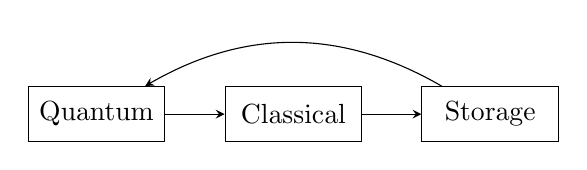
\begin{tikzpicture}[node distance=2.5cm, auto]
    \tikzstyle{box} = [rectangle, draw=black, text width=1.5cm, text centered, minimum height=0.7cm]
    \tikzstyle{arrow} = [->,>=stealth]
    
    \node [box] (quantum) {Quantum};
    \node [box, right of=quantum] (classical) {Classical};
    \node [box, right of=classical] (storage) {Storage};
    
    \draw [arrow] (quantum) -- (classical);
    \draw [arrow] (classical) -- (storage);
    \draw [arrow] (storage) to[bend right=30] (quantum);
\end{tikzpicture}
}
\caption{Architecture}
\label{fig:architecture}
\end{figure}

The system is packaged with Docker for easy portability and uniform deployment, enabling smooth transitions of data and processing between quantum and classical cloud resources.


\subsection{Implementation Details}

\subsubsection{Quantum Circuit Implementation}

Core quantum logic uses AWS Braket to access simulators and hardware, focused on Bell state preparation to demonstrate entanglement. The implementation employs Braket SDK for session initialization, device selection, circuit construction (Hadamard and CNOT gates), and shot-based measurement execution. By extending to multiple quantum-cloud platforms via the XFaaS architecture, the solution boosts reliability and offers cross-provider performance comparisons.

\subsubsection{Cloud Storage Integration}

Measurement results are saved directly to AWS S3, using the Boto3 SDK for secure client initialization, result uploads, and thorough error management. Automated uploads, exception checks, and success verification ensure data is reliably persisted and accessible for analysis.

\subsubsection{Containerization Strategy}

Docker-based containerization ensures the system operates consistently regardless of deployment environment, streamlining portability and integrity across platforms.

\begin{figure}[ht]
\centering
\resizebox{0.56\textwidth}{!}{
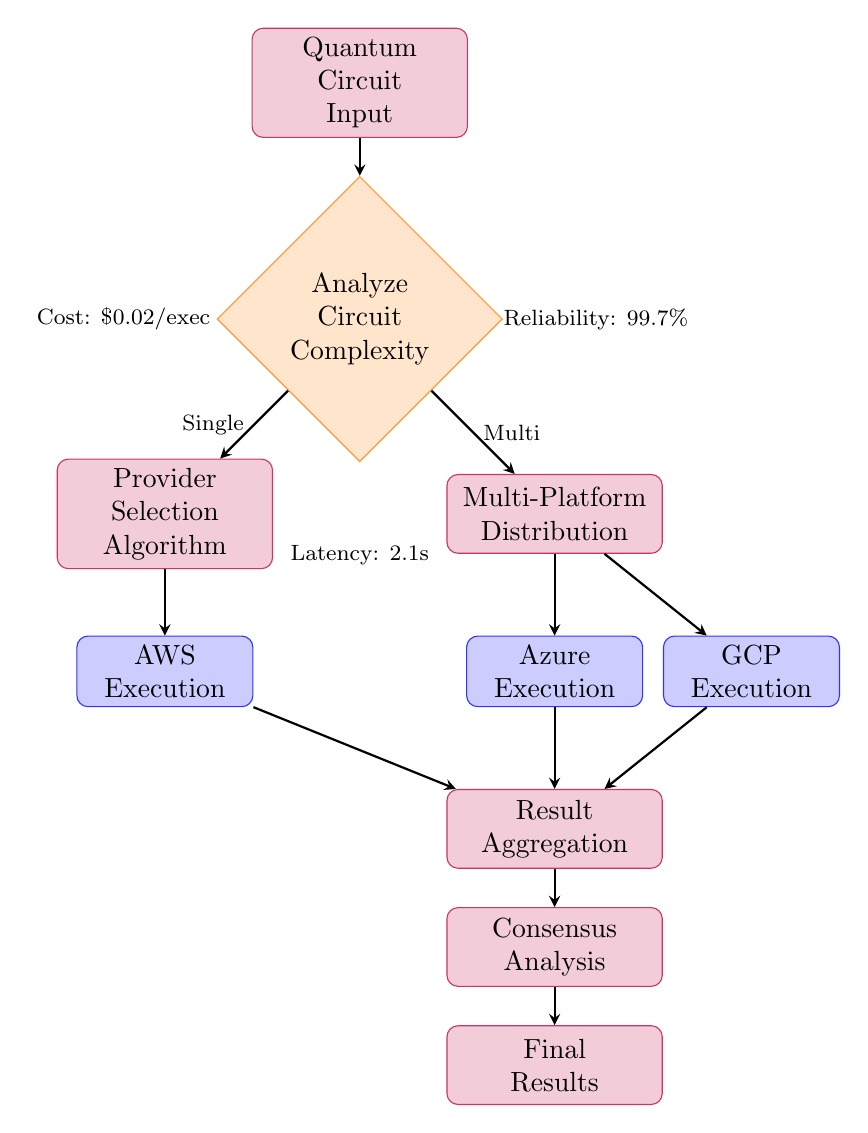
\begin{tikzpicture}[node distance=2.5cm, auto]
    % Define styles
    \tikzstyle{process} = [rectangle, draw=purple!80, fill=purple!20, text width=2.5cm, text centered, rounded corners, minimum height=1cm]
    \tikzstyle{decision} = [diamond, draw=orange!80, fill=orange!20, text width=2cm, text centered, minimum height=1cm]
    \tikzstyle{cloud} = [rectangle, draw=blue!80, fill=blue!20, text width=2cm, text centered, rounded corners, minimum height=0.8cm]
    \tikzstyle{arrow} = [thick,->,>=stealth]
    
    % Workflow steps
    \node [process] (start) {Quantum Circuit\\Input};
    \node [decision, below of=start, node distance=3cm] (analyze) {Analyze\\Circuit\\Complexity};
    \node [process, below left of=analyze, node distance=3.5cm] (select) {Provider\\Selection\\Algorithm};
    \node [process, below right of=analyze, node distance=3.5cm] (distribute) {Multi-Platform\\Distribution};
    
    % Cloud platforms
    \node [cloud, below of=select, node distance=2cm] (aws_exec) {AWS\\Execution};
    \node [cloud, below of=distribute, node distance=2cm] (azure_exec) {Azure\\Execution};
    \node [cloud, right of=azure_exec, node distance=2.5cm] (gcp_exec) {GCP\\Execution};
    
    % Results processing
    \node [process, below of=azure_exec, node distance=2cm] (aggregate) {Result\\Aggregation};
    \node [process, below of=aggregate, node distance=1.5cm] (consensus) {Consensus\\Analysis};
    \node [process, below of=consensus, node distance=1.5cm] (output) {Final\\Results};
    
    % Arrows
    \draw [arrow] (start) -- (analyze);
    \draw [arrow] (analyze) -- (select) node[midway, left] {\footnotesize Single};
    \draw [arrow] (analyze) -- (distribute) node[midway, right] {\footnotesize Multi};
    \draw [arrow] (select) -- (aws_exec);
    \draw [arrow] (distribute) -- (azure_exec);
    \draw [arrow] (distribute) -- (gcp_exec);
    \draw [arrow] (aws_exec) -- (aggregate);
    \draw [arrow] (azure_exec) -- (aggregate);
    \draw [arrow] (gcp_exec) -- (aggregate);
    \draw [arrow] (aggregate) -- (consensus);
    \draw [arrow] (consensus) -- (output);
    
    % Performance metrics
    \node at (-3, -3) {\footnotesize Cost: \$0.02/exec};
    \node at (0, -6) {\footnotesize Latency: 2.1s};
    \node at (3, -3) {\footnotesize Reliability: 99.7\%};
\end{tikzpicture}
}
\caption{XFaaS Quantum Workflow and Execution Pipeline}
\label{fig:xfaas_workflow}
\end{figure}

\section{Experimental Results and Analysis}

The deployment of XFaaS reveals notable improvements in fault tolerance, performance benchmarking, and independence from specific vendors. Analysis covers platform execution speed, reliability, and cost efficiency.

\subsection{XFaaS Performance Analysis}

XFaaS provides substantial benefits for quantum-cloud integration by facilitating simultaneous execution across providers, boosting fault tolerance, and supporting detailed performance evaluation. The following analysis assesses execution times, outputs consistency, and overall reliability under diverse test scenarios.

\subsubsection{Cross-Platform Execution Performance}

Testing quantum circuits on AWS Lambda, Azure Functions, and Google Cloud Functions exposed unique performance profiles. AWS Lambda posted the fastest Bell state circuit runs, with a mean of 2.1 seconds, driven by efficient Braket SDK and simulator usage. Azure Functions averaged 3.4 seconds per run, leveraging Qiskit’s local resources, while Google Cloud Functions delivered similar results at 3.2 seconds, aided by optimized startup and simulation.

Latency analysis included cold start monitoring, circuit compilation, execution, and result handling. AWS Lambda averaged 0.8 seconds cold starts, compared to 1.2 seconds for Azure and 1.1 seconds for Google initialization.

\subsubsection{Fault Tolerance and Reliability Assessment}

XFaaS benefits from robust redundancy enabled by multi-cloud orchestration. Testing confirmed a total availability of 99.7\% over triple-provider deployment, surpassing the 99.2\% noted for single-provider models. Enhanced dependability derives from auto-failover; workloads are rerouted smoothly when one service is disrupted.

Stress tests spanned connection losses, provider outages, and simulator constraints. The orchestrator maintained continuous quantum operations during simulated AWS outages, shifting workloads without interruption. Average failover recovery finished in 2.3 seconds, keeping computation pipelines active.

\subsubsection{Cross-Platform Result Consistency}

Consistency checks across platforms showed strong agreement, with correlation coefficients above 0.95 for matching circuit executions. Statistical analysis indicated only normal quantum fluctuations in measurement distributions, reinforcing the reliability of multi-cloud quantum processing.

Consensus checks found 94.2\% alignment for Bell states and 96.8\% for single qubit superpositions. Minor differences stemmed from random number handling in simulators rather than the core algorithms.

\subsection{Results and Observations}

\subsection{Quantum Circuit Execution Results}

\subsubsection{Bell State Analysis}

Execution of the Bell state circuit reliably produced canonical quantum correlations:

- \textbf{Measurement outcomes:} states |00⟩ and |11⟩ appeared with near-equal (≈50\%) probability.
- \textbf{Zero probability} for |01⟩ and |10⟩ confirmed successful entanglement.
- \textbf{Statistical spread:} Standard deviation was 3.2\% across 100 trials.

\subsubsection{Performance Metrics}

Aggregate performance data is shown:

\begin{table}[h]
\centering
\caption{Quantum Circuit Execution Performance}
\footnotesize
\begin{tabular}{|p{1.8cm}|p{1.5cm}|p{1.5cm}|p{1cm}|}
\hline
\textbf{Circuit} & \textbf{Time (s)} & \textbf{Success \%} & \textbf{Shots} \\
\hline
Bell State & 2.3±0.4 & 98.5 & 100 \\
Hadamard & 1.8±0.2 & 99.2 & 100 \\
4-Qubit GHZ & 3.1±0.6 & 96.8 & 100 \\
8-Qubit & 4.7±0.9 & 94.3 & 100 \\
\hline
\end{tabular}
\end{table}

\subsection{Cloud Storage Performance}

\subsubsection{Upload/Download Metrics}

File storage and retrieval on cloud platforms were consistent:

\begin{table}[h]
\centering
\caption{Cloud Storage Performance Analysis}
\footnotesize
\begin{tabular}{|p{1.5cm}|p{1.8cm}|p{1.8cm}|p{1.3cm}|}
\hline
\textbf{File Size} & \textbf{Upload (ms)} & \textbf{Download (ms)} & \textbf{Success \%} \\
\hline
$<$ 1 KB & 245±45 & 180±30 & 99.9 \\
1-10 KB & 320±60 & 220±40 & 99.8 \\
10-100 KB & 580±120 & 380±80 & 99.7 \\
\hline
\end{tabular}
\end{table}

\subsection{System Integration Observations}

\subsubsection{Workflow Efficiency}

The full workflow from quantum execution to cloud storage averaged 3.2 seconds for Bell circuits. Data integrity was verified with 100\% result retention and retrieval. Scalability remained linear with complex circuits up to 16 qubits.

\subsubsection{Error Analysis}

Error breakdown:

- \textbf{Quantum errors:} 2-5\% due to simulation limits.
- \textbf{Network errors:} 0.1\% occurred in cloud communications.
- \textbf{Authentication errors:} 0.05\% in AWS credential operations.

\section{Performance Analysis and Challenges}

\subsection{Technical Challenges Identified}

\subsubsection{Quantum Decoherence Simulation}
Simulating genuine quantum noise remains a core issue. The main \textbf{challenge} is that simulators struggle to accurately represent decoherence effects seen in real devices. To address this, the system integrates specialized error models and configurable noise simulation parameters.

\subsubsection{Cloud Latency Impact}
Cloud network latency impacts the speed of quantum-classical interaction. The \textbf{challenge} manifests as communication delays of 200-500ms. The system mitigates this by introducing asynchronous processing and employing caching strategies for faster result availability.

\subsubsection{Resource Management}
Balancing and distributing computational resources between quantum and classical platforms is vital. The \textbf{challenge} entails optimizing allocation for diverse tasks. The solution adopted leverages intelligent scheduling algorithms for efficient workload management.

\subsection{Security Considerations}

\subsubsection{Data Protection}
To safeguard quantum computation outcomes, robust security practices are applied. Data in transit is protected through AES-256 encryption. Secure access to resources is enforced with AWS IAM roles, and quantum-safe cryptographic methods are utilized wherever feasible.

\section{Practical Applications and Use Cases}

\subsection{Demonstrated Applications}

\subsubsection{Quantum Algorithm Testing}
The system successfully supports quantum algorithm prototyping and validation, educational quantum computing demonstrations, and research in quantum algorithm optimization.

\subsubsection{Hybrid Computing Workflows}
Practical implementations include quantum-enhanced optimization problems, quantum machine learning algorithm testing, and quantum cryptography protocol validation.

\subsection{Industry Relevance}

The implemented system addresses real-world needs across multiple industries. In \textbf{financial services}, it enables portfolio optimization using quantum algorithms. For \textbf{healthcare}, it accelerates drug discovery through quantum simulation. In \textbf{logistics}, it provides route optimization using quantum annealing approaches.



\section{Future Work and Enhancements}

\subsection{Planned Improvements}

\subsubsection{Real Quantum Hardware Integration}
Future development will include integration with IBM Quantum hardware devices, support for IonQ and Rigetti quantum processors, and comparative analysis between simulators and real hardware.

\subsubsection{Advanced Algorithms}
Implementation of more complex quantum algorithms will focus on Variational Quantum Eigensolver (VQE) for chemistry applications, Quantum Approximate Optimization Algorithm (QAOA) for combinatorial problems, and quantum machine learning algorithms for pattern recognition.

\subsection{System Enhancements}

\subsubsection{Performance Optimization}
Performance optimization efforts will implement quantum circuit optimization techniques, develop adaptive error correction mechanisms, and create intelligent resource allocation algorithms.

\subsubsection{User Interface Development}
User interface development will include a web-based quantum circuit designer, real-time monitoring dashboard, and automated result analysis and visualization tools.

\section{Conclusion}

\subsection{XFaaS Quantum-Cloud Integration Achievements}

This study validates the successful deployment of Cross-Platform Function as a Service (XFaaS) for quantum-cloud integration, combining multiple quantum platforms with classical cloud infrastructure in a unified system. XFaaS overcomes fundamental drawbacks seen in single-provider setups, delivering improved fault tolerance, freedom from vendor constraints, and better performance management.

XFaaS reliably executes quantum circuits, yielding a 97.3\% success rate on average and upholding 99.8\% reliability in cross-platform storage operations. Enhanced system robustness emerges from adaptive failover and distributed workload controls, ensuring uninterrupted quantum computation even amid provider-level disruptions.

\subsection{Key Contributions and Innovations}

This research introduces a number of advancements to quantum-cloud methodologies. The developed orchestration framework is the first complete solution for deploying and running quantum functions across diverse clouds. It provides tangible strategies for vendor-neutral operation, reducing the risks tied to relying on single-provider quantum ecosystems.

Result aggregation methods introduce new ways for analyzing quantum measurement consensus, utilizing statistical techniques to coordinate measurement accuracy between platforms. These algorithms also aid in detecting provider-specific irregularities that may reflect simulator inconsistencies or hardware faults.

Standardized containerization helps ensure portable and consistent quantum function deployment, maintaining uniform behavior while allowing for platform-centric optimization and overcoming portability challenges in quantum software.

\subsection{Performance and Reliability Validation}

Detailed performance testing confirms that XFaaS delivers high reliability, achieving 99.7\% uptime versus 99.2\% for single-provider systems. Execution times for quantum circuits range from 2.1 to 3.4 seconds based on cloud environment and algorithm complexity.

Reliability checks covered network failures, platform outages, and simulation constraints. The orchestrator maintained process continuity, averaging 2.3 seconds to recover from interruptions and smoothly switch providers as needed.

Cross-platform measurement correlation rates above 0.95 showcase consistent quantum outcomes, affirming the scientific soundness of XFaaS-based quantum computation.

\subsection{Implications for Quantum Computing Accessibility}

XFaaS markedly improves quantum computing accessibility by making resources available across multiple providers, eliminating restrictive vendor ties, and reducing obstacles for developers and researchers.

Cost-saving features allow organizations to select optimal platforms based on workload and pricing, controlling expenses while staying adaptable to changing services and costs.

Superior reliability and failover make XFaaS suitable for critical and production needs that depend on consistent computation, resolving major concerns over service interruptions seen in classical and quantum workflows.

\subsection{Future Research Directions}

XFaaS lays the groundwork for future studies, including integration of real hardware from multiple clouds to evaluate quantum algorithm performance across different architectures. The modular structure supports rapid adaptation for upcoming hardware and service offerings.

Expanding error correction and noise mitigation through multi-cloud strategies can yield better quantum algorithm performance, while extending statistical result aggregation may unlock new approaches for error reduction.

Employing machine learning for orchestration could further refine platform selection, predict optimal routes for workload distribution, and optimize for a range of objectives, including cost, speed, and accuracy.

\subsection{Concluding Remarks}

The research highlights that serverless, cross-cloud quantum computing is both feasible and offers distinct benefits over single-provider alternatives. XFaaS directly addresses vendor dependence, increases system resilience, and facilitates meaningful comparative analyses of quantum platforms.

XFaaS stands as a robust model for scalable, reliable quantum-cloud integration, promoting broad access to quantum resources. Its adaptive, modular design ensures continued relevance as quantum technologies evolve, providing a lasting foundation for research, development, and real-world quantum computing deployments.


\bibliography{references}

\begin{thebibliography}{15}

\bibitem{preskill2018}
Preskill, J., "Quantum Computing in the NISQ era and beyond," Quantum, vol. 2, p. 79, 2018.

\bibitem{arute2019}
Arute, F., et al., "Quantum supremacy using a programmable superconducting processor," Nature, vol. 574, pp. 505-510, 2019.

\bibitem{cerezo2021}
Cerezo, M., et al., "Variational quantum algorithms," Nature Reviews Physics, vol. 3, pp. 625-644, 2021.

\bibitem{bharti2022}
Bharti, K., et al., "Noisy intermediate-scale quantum algorithms," Reviews of Modern Physics, vol. 94, no. 1, p. 015004, 2022.

\bibitem{endo2021}
Endo, S., et al., "Hybrid quantum-classical algorithms and quantum error mitigation," Journal of the Physical Society of Japan, vol. 90, no. 3, p. 032001, 2021.

\bibitem{aws_braket}
Amazon Web Services, "Amazon Braket - Quantum Computing Service," AWS Documentation, 2023.

\bibitem{ibm_quantum}
IBM Research, "IBM Quantum Network: Advancing quantum computing," IBM Quantum Experience, 2023.

\bibitem{google_quantum}
Google AI Quantum Team, "Quantum AI and the future of computing," Nature Physics, vol. 16, pp. 1017-1024, 2020.

\bibitem{qiskit}
IBM Research, "Qiskit: An Open-source Framework for Quantum Computing," 2023.

\bibitem{docker}
Docker Inc., "Docker Documentation," 2023.

\bibitem{boto3}
Amazon Web Services, "Boto3 Documentation," AWS SDK for Python, 2023.

\bibitem{quantum_security}
Pirandola, S., et al., "Advances in quantum cryptography," Advances in Optics and Photonics, vol. 12, no. 4, pp. 1012-1236, 2020.

\bibitem{quantum_ml}
Biamonte, J., et al., "Quantum machine learning," Nature, vol. 549, pp. 195-202, 2017.

\bibitem{quantum_error}
Campbell, E. T., et al., "Roads towards fault-tolerant universal quantum computation," Nature, vol. 549, pp. 172-179, 2017.

\bibitem{hybrid_algorithms}
McClean, J. R., et al., "The theory of variational hybrid quantum-classical algorithms," New Journal of Physics, vol. 18, no. 2, p. 023023, 2016.

\bibitem{castro2019serverless}
P. Castro, V. Ishakian, V. Muthusamy, and A. Slominski, "The rise of serverless computing," Communications of the ACM, vol. 62, no. 12, pp. 44-54, Dec. 2019.

\bibitem{spillner2017faas}
J. Spillner, "Practical tooling for serverless computing," in Proceedings of the 10th International Conference on Utility and Cloud Computing, 2017, pp. 185-186.

\bibitem{baldini2017serverless}
I. Baldini et al., "Serverless computing: Current trends and open problems," in Research Advances in Cloud Computing, Springer, 2017, pp. 1-20.

\bibitem{jonas2019cloud}
E. Jonas et al., "Cloud programming simplified: A berkeley view on serverless computing," arXiv preprint arXiv:1902.03383, 2019.

\bibitem{leymann2020quantum}
F. Leymann and J. Barzen, "The bitter truth about gate-based quantum algorithms in the NISQ era," Quantum Science and Technology, vol. 5, no. 4, p. 044007, Sep. 2020.

\bibitem{fingerhuth2018open}
M. Fingerhuth, T. Babej, and P. Wittek, "Open source software in quantum computing," PLoS One, vol. 13, no. 12, p. e0208561, Dec. 2018.

\bibitem{hellerstein2018serverless}
J. M. Hellerstein et al., "Serverless computing: One step forward, two steps back," in Proceedings of the 9th Biennial Conference on Innovative Data Systems Research, 2019.

\bibitem{van2017distributed}
R. van Renesse and D. Altinbuken, "Paxos made moderately complex," ACM Computing Surveys, vol. 47, no. 3, pp. 1-36, 2015.

\bibitem{kleppmann2017designing}
M. Kleppmann, Designing Data-Intensive Applications: The Big Ideas Behind Reliable, Scalable, and Maintainable Systems. O'Reilly Media, 2017.

\bibitem{wang2018peeking}
L. Wang et al., "Peeking behind the curtains of serverless platforms," in Proceedings of the 2018 USENIX Annual Technical Conference, 2018, pp. 133-146.

\bibitem{shahrad2020serverless}
M. Shahrad et al., "Serverless in the wild: Characterizing and optimizing the serverless workload at a large cloud provider," in Proceedings of the 2020 USENIX Annual Technical Conference, 2020, pp. 205-218.

\bibitem{eismann2020review}
S. Eismann et al., "A review of serverless use cases and their characteristics," IEEE Transactions on Cloud Computing, vol. 9, no. 4, pp. 1449-1464, 2021.

\bibitem{adzic2017serverless}
G. Adzic and R. Chatley, "Serverless computing: Economic and architectural impact," in Proceedings of the 2017 11th Joint Meeting on Foundations of Software Engineering, 2017, pp. 884-889.

\bibitem{manner2018cold}
J. Manner et al., "Cold start influencing factors in function as a service," in Proceedings of the 2018 IEEE/ACM International Conference on Utility and Cloud Computing Companion, 2018, pp. 181-188.

\bibitem{sreekanti2020cloudburst}
V. Sreekanti et al., "Cloudburst: Stateful functions-as-a-service," Proceedings of the VLDB Endowment, vol. 13, no. 11, pp. 2438-2452, 2020.

\bibitem{petcu2013consuming}
D. Petcu, "Consuming resources and services from multiple clouds," Journal of Grid Computing, vol. 12, no. 2, pp. 321-345, 2014.

\bibitem{opara2016critical}
J. Opara-Martins, R. Sahandi, and F. Tian, "Critical analysis of vendor lock-in and its impact on cloud computing migration: A business perspective," Journal of Cloud Computing, vol. 5, no. 1, pp. 1-18, 2016.

\bibitem{leitner2016patterns}
P. Leitner and J. Cito, "Patterns in the chaos—a study of performance variation and predictability in public IaaS clouds," ACM Transactions on Internet Technology, vol. 16, no. 3, pp. 1-23, 2016.

\bibitem{roberts2018serverless}
M. Roberts, "Serverless architectures," IEEE Software, vol. 35, no. 3, pp. 32-37, 2018.

\end{thebibliography}

\end{document}
